\documentclass[11pt]{amsart}

\usepackage[T1]{fontenc}
\usepackage{lmodern}
\usepackage{amssymb,amsmath}
\usepackage{booktabs,array}
\usepackage{graphicx}
\usepackage[dvipsnames]{xcolor}
\usepackage[margin=1.15in]{geometry}
\usepackage[colorlinks=true,linkcolor=blue!50!black,citecolor=blue!50!black,urlcolor=blue!50!black]{hyperref}

\newtheorem{theorem}{Theorem}[section]
\newtheorem{proposition}[theorem]{Proposition}
\newtheorem{lemma}[theorem]{Lemma}
\newtheorem{corollary}[theorem]{Corollary}
\theoremstyle{definition}
\newtheorem{definition}[theorem]{Definition}
\newtheorem{innerconj}{Conjecture}
\newenvironment{conjecture}[1]{\renewcommand{\theinnerconj}{#1}\innerconj}{\endinnerconj}
\theoremstyle{remark}
\newtheorem{remark}[theorem]{Remark}

\numberwithin{equation}{section}

\newcommand{\davg}{\operatorname{deg_{avg}}}
\newcommand{\emo}{\operatorname{em}}
\newcommand{\Gb}{\overline{G}}
\hypersetup{pdftitle={A counterexample to a conjecture of Graffiti.pc on the forest number},pdfauthor={Deep Bhattacharjee}}
\providecommand{\doi}[1]{\url{https://doi.org/#1}}

\begin{document}

\title[A conjecture of Graffiti.pc on the forest number]{A counterexample to a conjecture\\ of Graffiti.pc on the forest number}

\author{Deep Bhattacharjee}
\address{Formerly, Electro-Gravitational Space Propulsion Laboratory (EGSPL),\newline Bhubaneswar, Odisha 751030, India}
\email{d.bhattacharjee@erl-forschung.de}
\email{itsdeep@live.com}
\urladdr{https://orcid.org/0000-0003-0466-750X}
\thanks{Corresponding author: \href{mailto:d.bhattacharjee@erl-forschung.de}{d.bhattacharjee@erl-forschung.de}; ORCID \href{https://orcid.org/0000-0003-0466-750X}{\mbox{0000-0003-0466-750X}}}

\subjclass[2020]{Primary 05C69; Secondary 05C05, 05C07}
\keywords{induced forest, forest number, degree sequence, complement, Graffiti.pc, counterexample}

\begin{abstract}
Conjecture 66 of Graffiti.pc bounds the order of a largest induced forest of a connected graph from below by the even mode of the degrees of its complement divided by its average degree. We show that it is false, under every reading of its definitions and by an unbounded margin.
\end{abstract}

\maketitle

\section{Introduction}

Graffiti.pc is a program written by DeLaVi\~na~\cite{DeLaVina2005} after Fajtlowicz's Graffiti~\cite{Fajtlowicz1988}; it proposes inequalities between graph invariants that hold on its database of graphs. DeLaVi\~na's list \emph{Written on the Wall~II}~\cite{WOWII} records its conjectures with their status. Conjecture~66, generated on 25 March 2004, is still marked as open (in the version of 26 July 2026). This note shows that it is false. The proofs are by hand; as in~\cite{BMB2026}, every finite statement is also re-checked by computer, and the counterexamples are also confirmed in the Lean proof assistant (Section~\ref{sec:search} and Appendix~\ref{app:verification}).

All graphs are finite and simple. For a graph $G$ with $n$ vertices and $m$ edges, $\davg(G)=2m/n$ is the average degree and $\Gb$ the complement, in which a vertex of degree $d$ in $G$ has degree $n-1-d$. The \emph{forest number} $f(G)$ is the largest number of vertices of an induced subgraph of $G$ that is a forest. The list defines the \emph{even mode} of a graph as ``the most frequently occurring degree that is an even integer'', with $\mathrm{even\_mode_{min}}$ the smallest one when several are equally frequent. We write $\emo(H)$ for this number: among the even values in the degree sequence of $H$, the most frequent one, and the smallest of these in case of a tie. Conjecture~66 reads as follows in~\cite{WOWII}.

\begin{conjecture}{66}\label{c66}
If $G$ is a simple connected graph, then
\[
f(G)\ \ge\ 2\left\lceil \frac{\emo(\Gb)}{\davg(G)}\right\rceil .
\]
\end{conjecture}

The definition of the even mode also admits a second reading: the smallest even value among the most frequent degrees, defined only when some most frequent degree is even. And while the statement uses $\lceil\cdot\rceil$, the definitions that the list attaches to it are those of $f$, the even mode, the complement, the average degree and the floor function $\lfloor\cdot\rfloor$. The list also records that in 2008 all $11{,}716{,}571$ connected graphs with $10$ vertices were added to the database of Graffiti.pc (see its notes to Conjectures~42 and~187). We show in Section~\ref{sec:search} that the printed conjecture fails on seven of these graphs, while the version with $\lfloor\cdot\rfloor$ holds on all of them; so the floor may well be what the program meant. We therefore treat all four readings.

For $c\ge1$ let $H_c$ be the graph made of $c$ disjoint copies $Q_1,\dots,Q_c$ of the complete graph $K_4$, with vertices $x_{i,0},x_{i,1},x_{i,2},x_{i,3}$ in $Q_i$, together with the $c-1$ edges $x_{i,1}x_{i+1,0}$ for $1\le i<c$ (Figure~\ref{fig:chain}).

\begin{theorem}\label{thm:main}
For every $c\ge1$, $f(H_c)=2c$, and the right side of Conjecture~\ref{c66} for $H_c$ equals $2\lceil q_c\rceil$ with
\[
q_c=\frac{8c(c-1)}{7c-1},
\]
under both readings of the even mode. Consequently Conjecture~\ref{c66} fails for $H_c$ if and only if $c\ge8$, and the conjecture with $\lfloor\cdot\rfloor$ in place of $\lceil\cdot\rceil$ fails for $H_c$ if and only if $c\ge14$. In both cases the right side exceeds $f(H_c)$ by at least $2\lfloor (c-7)/7\rfloor$, which tends to infinity.
\end{theorem}

\begin{theorem}\label{thm:search}
No connected graph with $2$ to $9$ vertices violates any of the four readings. Among the $11{,}716{,}571$ connected graphs with $10$ vertices, exactly $7$ violate Conjecture~\ref{c66} as printed, $5$ violate it when the even mode is read in the second way, and none violates either reading with $\lfloor\cdot\rfloor$.
\end{theorem}

The smallest member of the family that refutes all four readings, $H_{14}$, has $56$ vertices. We did not determine the smallest counterexample to the readings with $\lfloor\cdot\rfloor$; the smallest one we found has $37$ vertices (Remark~\ref{rem:37}).

\begin{figure}[t]
\centering
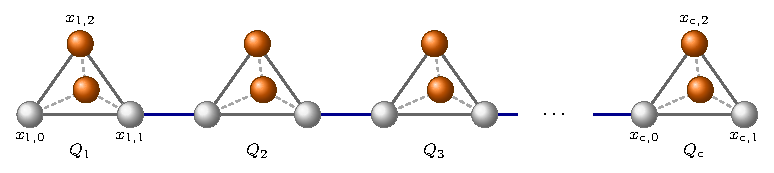
\includegraphics[width=0.92\textwidth]{figures/chain}
\caption{The graph $H_c$: copies $Q_1,\dots,Q_c$ of $K_4$, each drawn as a tetrahedron, joined by the edges $x_{i,1}x_{i+1,0}$. The shaded vertices $x_{i,2},x_{i,3}$ induce a forest of order $2c$.}
\label{fig:chain}
\end{figure}

\section{The chains of complete graphs}\label{sec:chain}

\begin{lemma}\label{lem:forest}
$f(H_c)=2c$.
\end{lemma}

\begin{proof}
Three vertices of one $Q_i$ induce a triangle, so an induced forest contains at most two vertices of each $Q_i$; since the $Q_i$ partition the vertex set, it has at most $2c$ vertices. The $2c$ vertices $x_{i,2},x_{i,3}$ induce $c$ disjoint edges, which form a forest.
\end{proof}

\begin{lemma}\label{lem:degrees}
$H_c$ is connected, has $7c-1$ edges, and $\davg(H_c)=(7c-1)/(2c)$. It has $2c+2$ vertices of degree $3$ and $2c-2$ vertices of degree $4$. In both readings the even mode of $\overline{H_c}$ equals $4c-4$.
\end{lemma}

\begin{proof}
The copies $Q_i$ are connected and consecutive ones are joined by an edge, so $H_c$ is connected; it has $6c$ edges inside the copies and $c-1$ between them. Every vertex has degree $3$ inside its copy, and the $2(c-1)$ endpoints $x_{i,1}$ $(i<c)$ and $x_{i,0}$ $(i>1)$ of the joining edges, which are distinct, have one more neighbour. In $\overline{H_c}$, which has $n=4c$ vertices, the degrees are therefore $4c-4$, which is even, taken $2c+2$ times, and $4c-5$, which is odd, taken $2c-2$ times. So $4c-4$ is the only even degree of $\overline{H_c}$, and it is also its most frequent degree, because $2c+2>2c-2$.
\end{proof}

\begin{lemma}\label{lem:arith}
Let $c\ge1$ and $q_c=8c(c-1)/(7c-1)$. Then $\lceil q_c\rceil\ge c+1$ if and only if $c\ge8$, and $\lfloor q_c\rfloor\ge c+1$ if and only if $c\ge14$. For $c\ge7$,
\[
\lfloor q_c\rfloor-c\ \ge\ \Bigl\lfloor\frac{c-7}{7}\Bigr\rfloor .
\]
\end{lemma}

\begin{proof}
We have
\[
q_c-c=\frac{8c^2-8c-7c^2+c}{7c-1}=\frac{c(c-7)}{7c-1}.
\]
Since $c$ is an integer, $\lceil q_c\rceil\ge c+1$ if and only if $q_c>c$, that is, $c>7$. Next, $q_c\ge c+1$ if and only if $c(c-7)\ge 7c-1$, that is, $c^2-14c+1\ge0$. The roots of $t^2-14t+1$ are $7\pm\sqrt{48}$, which lie in $(0,1)$ and $(13,14)$, so for positive integers $c$ this holds exactly when $c\ge14$. Finally, for $c\ge7$ we have $c/(7c-1)\ge1/7$ and $c-7\ge0$, so $q_c-c\ge(c-7)/7$, and taking integer parts gives the last claim.
\end{proof}

\begin{proof}[Proof of Theorem~\ref{thm:main}]
By Lemma~\ref{lem:degrees}, under either reading of the even mode,
\[
\frac{\emo(\overline{H_c})}{\davg(H_c)}=\frac{(4c-4)\cdot 2c}{7c-1}=q_c .
\]
By Lemma~\ref{lem:forest}, Conjecture~\ref{c66} fails for $H_c$ exactly when $2\lceil q_c\rceil>2c$, and the version with the floor fails exactly when $2\lfloor q_c\rfloor>2c$; Lemma~\ref{lem:arith} identifies these cases. The difference between the right side and $f(H_c)$ is at least $2\lfloor q_c\rfloor-2c\ge2\lfloor(c-7)/7\rfloor$.
\end{proof}

For example, $H_8$ has $32$ vertices, $f(H_8)=16$ and $q_8=448/55\approx8.15$, so the printed right side is $18$. For $H_{14}$, with $56$ vertices, $f(H_{14})=28$ and $q_{14}=1456/97\approx15.01$, so the right side is $32$ with $\lceil\cdot\rceil$ and $30$ with $\lfloor\cdot\rfloor$.

\begin{remark}
The family is close to extremal in the following sense. Alon, Kahn and Seymour~\cite{AKS1987} proved that $f(G)\ge\sum_v\min\{1,2/(d(v)+1)\}$, with equality for disjoint unions of complete graphs. For a connected graph whose degrees are all close to $d$, the right side of Conjecture~\ref{c66} is at most about $2n/d$ while $f(G)$ is at least about $2n/(d+1)$; a counterexample therefore needs the near-equality of disjoint cliques, a large even mode of the complement, and few extra edges to make the graph connected. The chains $H_c$ have all three.
\end{remark}

\begin{remark}\label{rem:37}
Let $T$ be the graph made of $12$ disjoint triangles $a_ib_ic_i$, the $11$ edges $b_ia_{i+1}$, and one pendant vertex attached to $a_1$. It has $37$ vertices and $48$ edges, $f(T)=25$ (at most two vertices of each triangle, and the pendant vertex), and the only even degree of $\overline T$ is $34$, taken by the $13$ vertices of degree $2$ in $T$. With the first reading of the even mode, $34/\davg(T)=34\cdot37/96\approx13.10$, so the right side is $26$ with $\lfloor\cdot\rfloor$ and $28$ with $\lceil\cdot\rceil$. The most frequent degree of $\overline T$ is the odd number $33$, so $T$ says nothing about the second reading.
\end{remark}

\section{Small graphs}\label{sec:search}

Let $G_{10}$ be the graph obtained from a triangle $t_1t_2t_3$ and a complete graph on $\{q_1,q_2,q_3,q_4\}$ by adding the edge $t_1q_1$ and three pendant vertices $\ell_1,\ell_2,\ell_3$, with $\ell_i$ adjacent to $q_i$ (Figure~\ref{fig:g10}).

\begin{proposition}\label{prop:g10}
$G_{10}$ is a counterexample to Conjecture~\ref{c66} as printed, under both readings of the even mode: $f(G_{10})=7$, while the right side is $8$.
\end{proposition}

\begin{proof}
An induced forest contains at most two vertices of the triangle, at most two of the $K_4$, and the three pendant vertices, so $f(G_{10})\le7$; the seven shaded vertices in Figure~\ref{fig:g10} induce the forest $t_2t_3$, $\ell_2q_2q_3\ell_3$, $\ell_1$. The degrees of $G_{10}$ are $5$ ($q_1$), $4$ ($q_2,q_3$), $3$ ($t_1,q_4$), $2$ ($t_2,t_3$) and $1$ ($\ell_1,\ell_2,\ell_3$); so $m=13$, $\davg(G_{10})=13/5$, and the degrees of $\overline{G_{10}}$ are $4,5,5,6,6,7,7,8,8,8$. The value $8$ occurs three times and every other value at most twice, so it is the even mode under both readings, and the right side is $2\lceil 8\cdot5/13\rceil=2\lceil40/13\rceil=8$.
\end{proof}

With $\lfloor\cdot\rfloor$ the right side for $G_{10}$ is $2\lfloor40/13\rfloor=6$, and the inequality holds.

\begin{figure}[t]
\centering
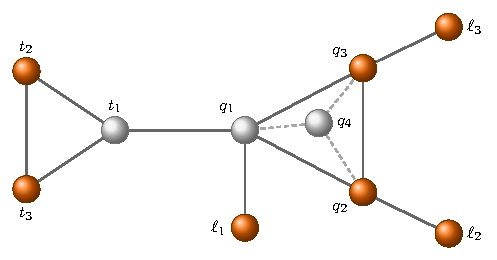
\includegraphics[width=0.62\textwidth]{figures/g10}
\caption{The graph $G_{10}$. The shaded vertices induce a forest of order $7=f(G_{10})$.}
\label{fig:g10}
\end{figure}

Theorem~\ref{thm:search} comes from an exhaustive search. The connected graphs with at most $10$ vertices were generated with \texttt{geng} from nauty~\cite{McKayPiperno2014}, and for each of them the four right sides were computed in integer arithmetic (the quotient $x/\davg(G)$ equals $xn/(2m)$) and compared with the forest number, computed by branch and bound over vertex subsets. Table~\ref{tab:search} gives the results. The seven counterexamples with $10$ vertices all have $13$ edges, three pendant vertices and forest number $7$; their graph6 codes are \texttt{I?ACJ@PqW} (this is $G_{10}$), \texttt{I?AACJafO}, \texttt{I?AACIdu\_}, \texttt{I?AADJAfO}, \texttt{I?AADHQbW}, \texttt{I?ABAeKOw} and \texttt{I?{}\textasciigrave{}CR@PoW}, and the last two violate only the first reading of the even mode.

\begin{table}[t]
\centering
\caption{Counterexamples among the connected graphs with $n$ vertices. A dash means that no graph of that order has an even mode under the reading, or none violates it; the readings are the even mode as defined (first) or as the smallest even most frequent degree (second), each with $\lceil\cdot\rceil$ or $\lfloor\cdot\rfloor$.}
\label{tab:search}
\begin{tabular}{rrcccc}
\toprule
$n$ & graphs & first, $\lceil\cdot\rceil$ & second, $\lceil\cdot\rceil$ & first, $\lfloor\cdot\rfloor$ & second, $\lfloor\cdot\rfloor$\\
\midrule
$2$--$8$ & $12{,}112$ & $0$ & $0$ & $0$ & $0$\\
$9$ & $261{,}080$ & $0$ & $0$ & $0$ & $0$\\
$10$ & $11{,}716{,}571$ & $7$ & $5$ & $0$ & $0$\\
\bottomrule
\end{tabular}
\end{table}

\appendix

\section{Verification}\label{app:verification}

The proofs above use no computation. The computer checks the finite claims and the search of Section~\ref{sec:search}, independently in C, C++, Bash, Python, Julia and Lean; all files are in the repository listed under Data and code availability, where \texttt{scripts/run\_all.sh} runs them.
\begin{enumerate}
\item \textbf{C.} \texttt{wowii66.c} performs the search of Section~\ref{sec:search} on graph6 input, and for $c\le300$ builds $H_c$ and checks Lemmas~\ref{lem:forest}--\ref{lem:arith}: the degrees, the even modes and both right sides, the partition into cliques and the explicit forest of order $2c$, and $f(H_c)=2c$ by branch and bound for $c\le6$.
\item \textbf{C++.} \texttt{wowii66.cpp} repeats both computations with no shared code and a different method for $f$ (a greedy lower bound, and an exact value over all vertex subsets only when that bound is below the right side). Its output for all connected graphs with at most $10$ vertices is identical, line for line, to that of the C program.
\item \textbf{Bash} (shell integer arithmetic only): $G_{10}$, with $f(G_{10})=7$ over all $1024$ vertex subsets; $H_c$ for $c\le40$; and the inequalities of Lemma~\ref{lem:arith} for $c\le20000$.
\item \textbf{Python} (exact rational arithmetic): $G_{10}$ and the seven graphs of Table~\ref{tab:search}, with $f$ over all vertex subsets and a colour-refinement check that the seven are pairwise non-isomorphic; every labelled connected graph with at most $6$ vertices; $H_c$ for $c\le60$, with $f$ over all subsets for $c\le4$; and the inequalities of Lemma~\ref{lem:arith} for $c\le10^5$.
\item \textbf{Julia} (exact rational arithmetic): the same graphs, $H_c$ for $c\le300$, and $f(H_c)=2c$ over all $2^{4c}$ vertex subsets for $c\le5$.
\item \textbf{Lean~4}~\cite{MouraUllrich2021}: a self-contained file without Mathlib computes, in the kernel, every quantity of Proposition~\ref{prop:g10} from the edge list of $G_{10}$, including $f(G_{10})=7$ over all $1024$ vertex subsets, and proves that Conjecture~\ref{c66} fails for $G_{10}$ under both readings; the proof depends only on the axiom \texttt{propext}.
\item \textbf{Lean~4 with Mathlib}~\cite{Mathlib2020}: a second file defines the forest number, both readings of the even mode and the average degree for every finite simple graph, and proves for every $c$ that $H_c$ is connected, that $f(H_c)\le2c$, the degrees of $\overline{H_c}$, both even modes and both right sides. It concludes that $H_c$ violates Conjecture~\ref{c66} under both readings for every $c\ge8$, and the version with $\lfloor\cdot\rfloor$ for every $c\ge14$. The proof uses only the standard axioms \texttt{propext}, \texttt{Classical.choice} and \texttt{Quot.sound}.
\end{enumerate}

\section*{Statements and Declarations}

\subsection*{Funding} No funding was received for conducting this study.

\subsection*{Competing interests} The author has no competing interests to declare that are relevant to the content of this article.

\subsection*{Data and code availability} The programs, their outputs and the Lean files are available at \url{https://github.com/creelie/eConjectureWOWII66} and archived on Zenodo, \doi{10.5281/zenodo.23254096}.

\subsection*{Use of generative AI} The author used Claude (Anthropic) for programming, computation and drafting; the author checked the mathematics and takes full responsibility for the content.

{\raggedright
\begin{thebibliography}{99}

\bibitem{AKS1987}
N.~Alon, J.~Kahn and P.~D. Seymour, \emph{Large induced degenerate subgraphs}, Graphs Combin. \textbf{3} (1987), 203--211. \doi{10.1007/BF01788542}

\bibitem{BMB2026}
D.~Bhattacharjee, P.~Mandal and U.~Bhattacharya, \emph{Resolving Erd\H{o}s--Ulam monochromatic union-closed family conjectures}, preprint, 2026. \href{https://arxiv.org/abs/2610.02833}{arXiv:2610.02833}

\bibitem{DeLaVina2005}
E.~DeLaVi\~na, \emph{Graffiti.pc: a variant of Graffiti}, in: Graphs and Discovery, DIMACS Ser. Discrete Math. Theoret. Comput. Sci. 69, Amer. Math. Soc., Providence, RI, 2005, 71--79. \doi{10.1090/dimacs/069/05}

\bibitem{WOWII}
E.~DeLaVi\~na, \emph{Written on the Wall II (conjectures of Graffiti.pc)}, \url{http://cms.uhd.edu/faculty/delavinae/research/wowII/}; version of 26 July 2026 archived at \url{https://web.archive.org/web/20260726061534/http://cms.uhd.edu/faculty/delavinae/research/wowII/all.html}

\bibitem{Fajtlowicz1988}
S.~Fajtlowicz, \emph{On conjectures of Graffiti}, Discrete Math. \textbf{72} (1988), 113--118. \doi{10.1016/0012-365X(88)90199-9}

\bibitem{Mathlib2020}
The mathlib Community, \emph{The Lean mathematical library}, in: Proceedings of the 9th ACM SIGPLAN International Conference on Certified Programs and Proofs (CPP 2020), ACM, New York, 2020, 367--381. \doi{10.1145/3372885.3373824}

\bibitem{McKayPiperno2014}
B.~D. McKay and A.~Piperno, \emph{Practical graph isomorphism, II}, J. Symbolic Comput. \textbf{60} (2014), 94--112. \doi{10.1016/j.jsc.2013.09.003}

\bibitem{MouraUllrich2021}
L.~de Moura and S.~Ullrich, \emph{The Lean 4 theorem prover and programming language}, in: Automated Deduction -- CADE 28, Lecture Notes in Comput. Sci. 12699, Springer, Cham, 2021, 625--635. \doi{10.1007/978-3-030-79876-5_37}

\end{thebibliography}
}

\end{document}
